% --------------------------------------------------------------
% This is all preamble stuff that you don't have to worry about.
% Head down to where it says "Start here"
% --------------------------------------------------------------

\documentclass[12pt]{article}

\usepackage[margin=1in]{geometry}
\usepackage{amsmath,amsthm,amssymb}
\usepackage{graphicx}
\usepackage{subcaption}
\usepackage{algorithmicx}
\usepackage{algorithm}
\usepackage{algpseudocode}
\usepackage[colorlinks,linkcolor=blue]{hyperref}
\usepackage[noabbrev]{cleveref}
\usepackage{courier}
\usepackage{listings}


\oddsidemargin 0in
\evensidemargin 0in
\textwidth 6.5in
\topmargin -0.5in
\textheight 9.0in

\newcommand{\ignore}[1]{}
\def\pp{\par\noindent}

\newcommand{\assignment}[4]{
\thispagestyle{plain}
\newpage
\setcounter{page}{1}
\noindent
\begin{center}
\framebox{ \vbox{ \hbox to 6.28in
{CIS 4190/5190: Applied Machine Learning \hfill #1}
\vspace{4mm}
\hbox to 6.28in
{\hspace{2.5in}\large\bf\mbox{Homework #2}}
\vspace{4mm}
\hbox to 6.28in
{{\it Handed Out: #3 \hfill Due: #4}}
}}
\end{center}
}

\makeatletter
\renewcommand{\fnum@algorithm}{\fname@algorithm}
\makeatother

\lstset{basicstyle=\footnotesize\ttfamily,breaklines=true}
\lstset{framextopmargin=50pt,frame=bottomline}


\begin{document}

\assignment{Spring 2023}{2}{January 25}{February 8}

% --------------------------------------------------------------
%                         Start here
% --------------------------------------------------------------


{\bf Name: }  Qihang Dai\\

{\bf PennKey:} ahgdyyycc\\

{\bf PennID:} 78803164\\

Note: This document is a read-only file. To create an editable version click on Menu in the top left corner of your screen and choose the Copy Project option. 
\section{Multiple Choice \& Written Questions}

\begin{enumerate}
\item
\begin{enumerate}
\item decrease bias and increase variance
\item increase bias and decrease variance
\item decrease bias and increase variance
\end{enumerate}
This means the modle is overfitting: low bias and high variance. thus we want a more generalized modle and a more simple prediciton.
Thus we increase n, decrease $\lambda$, and decrease d.

\item (A) global maxium

\item
\begin{enumerate}
\item $$\frac{\partial R_1}{\partial B_j} = \lambda sgn(B_j)$$
$$\frac{\partial R_2}{\partial B_j} = 2 \lambda B_j^2$$
\item since L1 regularization's gradient is independent of $w$, it will do a better job to push weight to zero when weight is small. 
\end{enumerate} 

\item
\begin{enumerate}
\item since x $>$ 0, we have a = 1 and b = 0. y = x\\ 
for x distribution on [-1, 0], we have:
\begin{flalign}
MSE &= \frac{1}{n}\sum_{i=1}^n (x_i - 0)^2\\
&= \frac{1}{n}\sum_{i=1}^n x_i^2\\
&= \int_{-1}^{0} x^2 \,dx \\
&= \frac{1}{3}
\end{flalign}
\item the learned model should be y = 0 (a = 0 and b = 0). for MSE on X ~ U[0, 1], we have: y = x and MSE is still $\frac{1}{3}$
\end{enumerate}

\item 
\begin{gather*} 
    f_{\hat{\beta}}(x) = \hat{\beta}^T x  = x ^ T \hat{\beta} \\
    \hat{\beta} = (X^T X)^{-1} X^T Y \\
    f_{\hat{\beta}}(x) = x^T (X^T X)^{-1} X^T Y \\
    Y = (y1, y2, ..., yn)^T, we have \\
    f_{\hat{\beta}}(x) = x^T (X^T X)^{-1} X^T (y1, y2, ..., yn)^T \\
    = \sum_{i=1}^n x^T (X^T X)^{-1} X^T yi \\
    k_i = x^T (X^T X)^{-1} X^T I_i
\end{gather*}
$I_i$ represent (d x 1) vector where only ith element is 1 and others are 0.
\end{enumerate}

\section{Python Programming Questions}

TODO: Please add the resulting plots for Question 1.3 and Question 1.4.

\begin{figure}
\centering
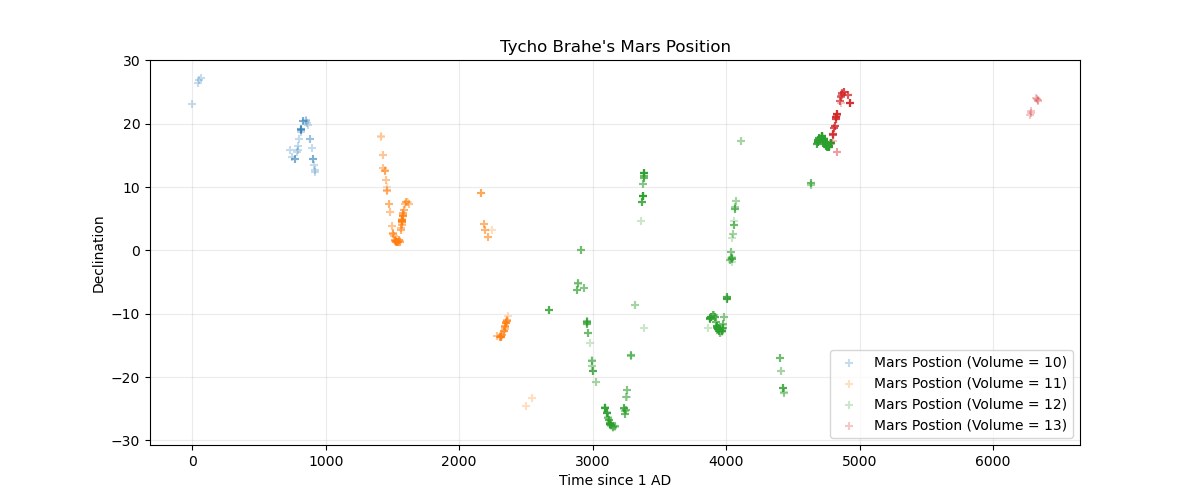
\includegraphics[width=0.8\textwidth]{example-figure.png}
\caption{Figure}
\end{figure}

\end{document} 